\chapter{Implementación del sistema}
\label{chap:implementacion}

\lettrine{E}{n} este capítulo se describe el estado de implementación del sistema según la arquitectura modular definida, diferenciando claramente lo implementado de las líneas de evolución.

\section{Visión general del estado actual}

La implementación actual cubre un flujo funcional extremo a extremo en entorno local:

\begin{itemize}
  \item captura de datos inerciales en Android;
  \item gestión local de sesiones;
  \item integración con ESP32 para control de captura y descarga;
  \item visualización operativa de sesiones desde la aplicación.
\end{itemize}

La capa backend remota se mantiene como fase de evolución y no como componente cerrado en el estado actual.

\section{Implementación del modo móvil en Android}

El modo móvil registra sensores inerciales del teléfono y guarda las capturas como sesiones en almacenamiento de la app.
Cada sesión incluye muestras temporales y metadatos mínimos para trazabilidad.

\subsection{Captura y persistencia local}

La app implementa captura con duración configurable y guardado automático en ficheros de sesión.
Esta decisión permite trabajar sin infraestructura externa en etapas tempranas y facilita depuración rápida.

\subsection{Gestión de sesiones}

Se implementan operaciones de catálogo para listar, renombrar, eliminar y abrir sesiones.
Esto convierte la app en una herramienta operativa de trabajo y no solo en una pantalla de captura puntual.

\section{Implementación del modo ESP32}

La integración embebida se implementa como flujo de operación desde Android contra el nodo ESP32.
El intercambio actual se realiza por red local, con endpoints para verificación de estado, control de captura y descarga de datos.

\subsection{Flujo de operación embebida}

La app permite:

\begin{itemize}
  \item comprobar conectividad con el nodo;
  \item iniciar/parar captura remota;
  \item descargar sesión generada en el ESP32;
  \item almacenar y visualizar la sesión de forma homogénea al modo móvil.
\end{itemize}

Este diseño mantiene una experiencia operativa consistente entre ambos orígenes de datos.

\subsection{Firmware del ESP32}

El firmware actual incluye funciones de red, estado de captura y descarga de sesiones.
Además, incorpora soporte de diagnóstico y un modo de simulación para acelerar pruebas cuando la integración física del sensor no está cerrada.

\section{Contrato de sesión y formato de datos}

El sistema utiliza una sesión como unidad de trabajo compartida.
En la implementación actual, el formato local de referencia está orientado a series temporales con metadatos básicos.

Se mantiene como criterio de diseño que la sesión contenga identidad de origen, base temporal y parámetros de captura suficientes para comparación y reprocesado.

\section{Visualización y explotación en la app}

La aplicación integra visualización de sesiones y panel de estado de operación.
El objetivo principal de esta capa es permitir inspección rápida, trazabilidad de capturas y flujo de trabajo continuo (captura, revisión, gestión y exportación).

\begin{figure}[htbp]
  \centering
  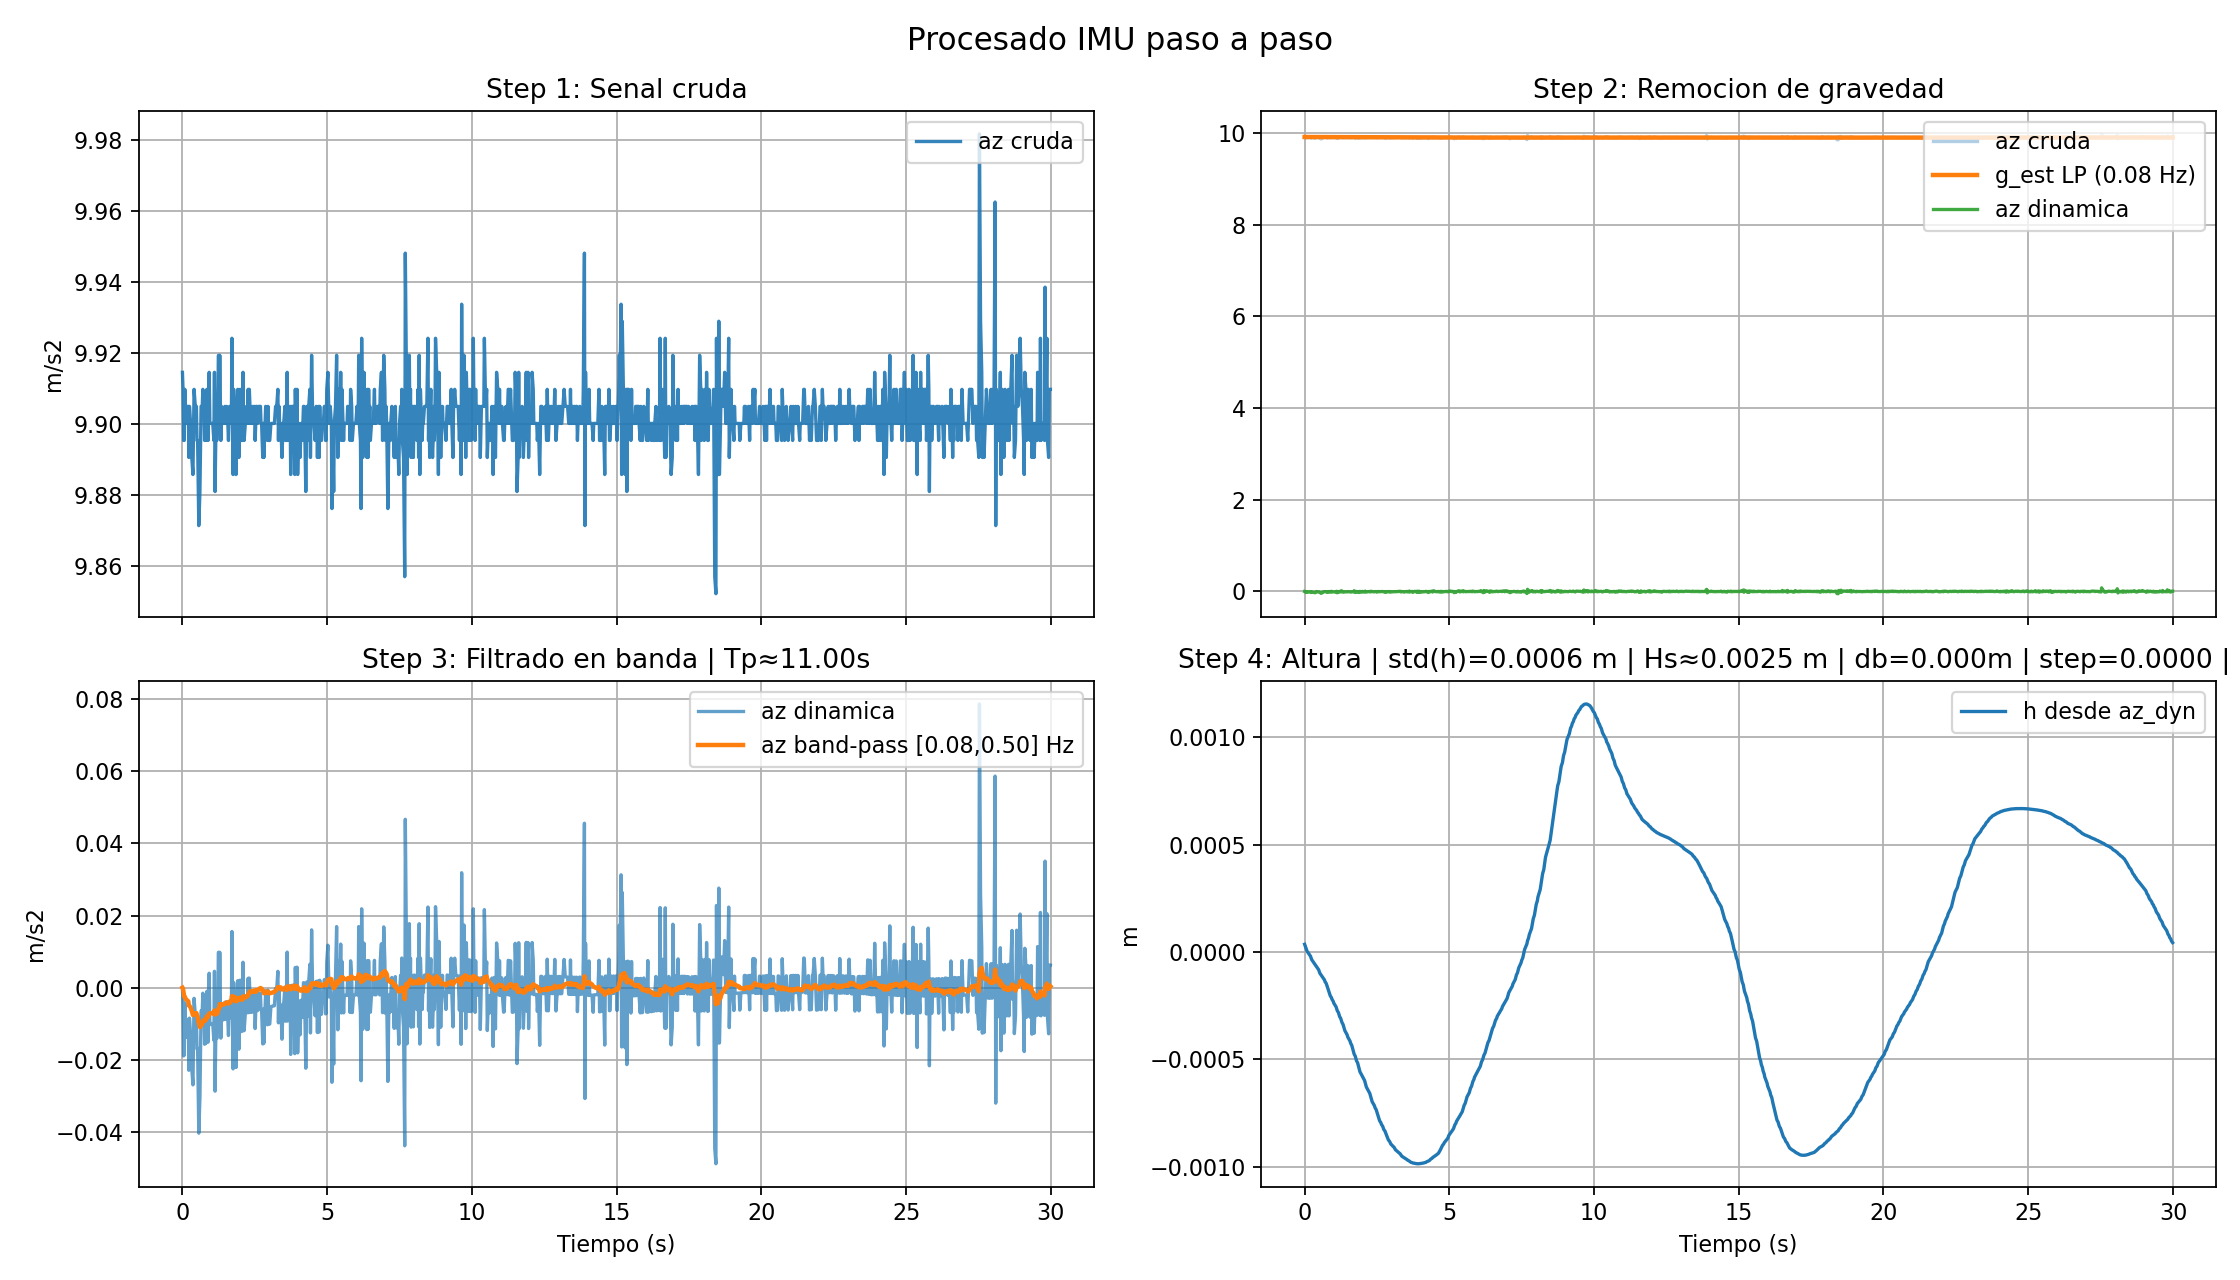
\includegraphics[width=0.95\textwidth]{imaxes/imu_pipeline_all.png}
  \caption{Vista de apoyo utilizada para revisión de sesiones y depuración del flujo de datos.}
  \label{fig:imu-pipeline-all}
\end{figure}

\section{Diseño software y desacoplamiento}

A nivel de implementación, se mantiene separación entre:

\begin{itemize}
  \item captura;
  \item repositorio de sesiones;
  \item comunicación con nodo embebido;
  \item visualización y operación.
\end{itemize}

Esta separación reduce acoplamiento y facilita introducir backend remoto o cambios de transporte sin rehacer la aplicación.

\section{Estado de backend remoto}

La integración con backend cloud se considera una fase posterior del desarrollo.
En esta etapa, se mantienen definidos los requisitos de capa remota (sincronización de sesiones, estado de nodos y acceso externo), dejando abierta la elección tecnológica final.

\section{Herramientas de soporte de ingeniería}

Durante el desarrollo se han utilizado scripts y utilidades de diagnóstico para acelerar verificación de captura, comunicación y consistencia de sesiones.
Estas herramientas se consideran apoyo técnico de implementación y no sustituyen al flujo de producto principal en Android.

\section{Limitaciones del estado implementado}

En el estado actual del TFG, las limitaciones más relevantes son:

\begin{itemize}
  \item dependencia de operación local para parte del flujo embebido;
  \item backend remoto todavía no integrado en la rama principal;
  \item necesidad de consolidar validación comparativa completa bajo protocolo homogéneo.
\end{itemize}

Estas limitaciones se asumen explícitamente como parte de un desarrollo incremental orientado a reducir riesgo técnico.
